%% Based on a TeXnicCenter-Template, which was
%% created by Christoph B�rensen
%% and slightly modified by Tino Weinkauf.
%%%%%%%%%%%%%%%%%%%%%%%%%%%%%%%%%%%%%%%%%%%%%%%%%%%%%%%%%%%%%

\documentclass[a4paper,12pt]{scrartcl} %This is a special class provided by the KOMA script, which does a lot of adjustments to adapt the standard LaTeX classes to european habits, change to [a4paper,12pt,twoside] for doublesided layout


%########################### Preferences #################################


% ******** vmargin settings *********
\usepackage{vmargin} %This give you full control over the used page arae, it maybe not the idea od Latex to do so, but I wanted to reduce to amount of white space on the page
\setpapersize{A4}
\setmargins{3.5cm}%			%linker Rand, left edge
					 {1.5cm}%     %oberer Rand, top edge
           {14.7cm}%		%Textbreite, text width
           {23.42cm}%   %Texthoehe, text hight
           {14pt}%			%Kopfzeilenh�he, header hight
           {1cm}%   	  %Kopfzeilenabstand, header distance
           {0pt}%				%Fu�zeilenhoehe footer hight
           {2cm}%    	  %Fusszeilenabstand, footer distance         

% ********* Font definiton ************
\usepackage{t1enc} % as usual
\usepackage[latin1]{inputenc} % as usual
\usepackage{times}
\usepackage[utf8]{inputenc}		
%\usepackage{mathptmx}  	%mathematical fonts for use with times, I encountered some problems using this package togather with pdftex, which I was not able to resolve
% ********* Graphics definition *******

\usepackage[pdftex]{graphicx} % required to import graphic files
\usepackage{color} %allows to mark some entries in the tables with color
\usepackage{eso-pic} % these two are required to add the little picture on top of every page
\usepackage{everyshi} % these two are required to add the little picture on top of every page
\renewcommand{\floatpagefraction}{0.7} %default:0.5 allows two big pictures on one page

%********** Enybeling Hyperlinks *******
\usepackage[pdfborder=000,pdftex=true]{hyperref}% this enables jumping from a reference and table of content in the pdf file to its target

% ********* Table layout **************
\usepackage{booktabs}	  	%design of table, has an excellent documentation
%\usepackage{lscape}			%use this if you want to rotate the table together with the lines around the table

% ********* Caption Layout ************
\usepackage{ccaption} % allows special formating of the captions
\captionnamefont{\bf\footnotesize\sffamily} % defines the font of the caption name (e.g. Figure: or Table:)
\captiontitlefont{\footnotesize\sffamily} % defines the font of the caption text (same as above, but not bold)
\setlength{\abovecaptionskip}{0mm} %lowers the distace of captions to the figure


% ********* Header and Footer **********
% This is something to play with forever. I use here the advanced settings of the KOMA script

\usepackage{scrpage2} %header and footer using the options for the KOMA script
\renewcommand{\headfont}{\footnotesize\sffamily} % font for the header
\renewcommand{\pnumfont}{\footnotesize\sffamily} % font for the pagenumbers

%the following lines define the pagestyle for the main document
\defpagestyle{cb}{%
(\textwidth,0pt)% sets the border line above the header
{\pagemark\hfill\headmark\hfill}% doublesided, left page
{\hfill\headmark\hfill\pagemark}% doublesided, right page
{\hfill\headmark\hfill\pagemark}%  onesided
(\textwidth,1pt)}% sets the border line below the header
%
{(\textwidth,1pt)% sets the border line above the footer
{{\it RTMA 1 }\hfill Universit� de Poitiers}% doublesided, left page
{Universit� de Poitiers\hfill{\it RTMA 1}}% doublesided, right page
{RTMA 1\hfill{\it Universit� de Poitiers}} % one sided printing
(\textwidth,0pt)% sets the border line below the footer
}

%this defines the page style for the first pages: all empty
\renewpagestyle{plain}%
	{(\textwidth,0pt)%
		{\hfill}{\hfill}{\hfill}%
	(\textwidth,0pt)}%
	{(\textwidth,0pt)%	
		{\hfill}{\hfill}{\hfill}%
	(\textwidth,0pt)}

%********** Footnotes **********
\renewcommand{\footnoterule}{\rule{5cm}{0.2mm} \vspace{0.3cm}} %increases the distance of footnotes from the text
\deffootnote[1em]{1em}{1em}{\textsuperscript{\normalfont\thefootnotemark}} %some moe formattion on footnotes

%################ End Preferences, Begin Document #####################

\pagestyle{plain} % on headers or footers on the first page

\begin{document}

\begin{center}

\begin{figure}[th]
    \centering
		
\includegraphics[width=10cm]{Universite_de_Poitiers_logo.jpg}
	\label{fig:logo}
\end{figure}

\vspace{2cm}

% There might be better solutions for the title page, giving all distances and sizes manually was simply the easiest solution
{\Large\bf\sf UFR Sciences fondamentales et appliqu�es}%as this is an english text I didn't load the german package, this would ease the use of special characters
\vspace{2cm}
{\Huge\bf\sf Algorithmic tools and software  }

\vspace{.5cm}

{\Huge\bf\sf for facial recognition}

%\vspace{.5cm}

%{\Huge\bf\sf to use with TeXnicCenter}

\vspace{2cm}



{\Large\bf\sf \today} %adds the current date

\vspace{\fill}

{\Large\bf\sf Master 1 RTMA 2014/2015

\end{center}
\newpage

%%The following loads the picture on top of every page, the numbers in \put() define the position on the page:
%\AddToShipoutPicture{\setlength\unitlength{0.1mm}\put(604,2522){
\includegraphics[width=1.5cm]{logo.jpg}}}

\pagestyle{cb} % now we want to have headers and footers

\tableofcontents

\newpage

\section{Project environment} 
\subsection{Context and environment}
Previously carried out at the SIC Department of XLIM laboratory, the project we are in charge of implements "algorithmic tools and capturing software for facial recognition". This project interest was also interactions with and between users of a video game with an educational aim ("Serious game") by automatically animated avatars and experienced analysis difficulties, as well as the development of a software library for developers of video games on smartphones.
Facial recognition is often used as a tool to secure devices or control the use of applications. This technique both helps adults secure their systems and devices and parents limit and control access to systems for their kids.
The main idea was to improve parental control of tablets for children�s use. This could be helpful for parents wishing to use facial recognition to limit their children�s use past a certain time of a day.
 
\subsection{Project Objective}
The work required for this project is the development of a share recording software for the recognition of facial expressions for the identification of a face from an ID list in a home or for parental control.
Today innovation and the latest technologies are growing increasingly and allow the interactivity between human-machine to be maximal. Research  on facial expression is fundamental in many applications.
Facial recognition takes place in three stages, namely:
		\begin{itemize}
		\item Face detection ;
		\item Extraction and normalization of facial features ;
		\item Identification and / or verification.
		\end{itemize}

The main difficulty in face recognition is that  there are no two identical faces. Thus, each individual is unique and will be marked by gender, ethnicity, age or his haircut, but also by the shape, size and arrangement of the elements of the face.
This project has an educational goal because it contributes greatly to our engineering multimedia training, allowing us to put into practice the theories studied in the various teaching modules of our maste�sr degree (Image processing, tool and scientific computation, Algorithms for multimedia, random signal processing) but also by completing them. This project can be seen as a complement to our training.

\subsection{Needs analysis}

This project aims to develop a facial capture software program (face recognition) in XLIM-SIC laboratory research work in collaboration with a company based in Lyon operating in the field of manufacturing tablets for children .
The required results at the end of this project are: facial recognition software program with
		
		\begin{itemize}
		\item Eigen Faces;
		\item Fisher Faces.
		\end{itemize}


Those will be programmed with multiple programming languages (Python, C ++).
This project is performed with the research professors of the Fundamental Faculty of  Sciences at the University of Poitiers: Pascal Bourdon and David HELBERT who  supervises the project.

\subsection{Actors}
Those will be programmed with multiple programming languages (Python, C ++).
This project is performed with the research professors of the Fundamental Faculty of  Sciences at the University of Poitiers: Pascal Bourdon and David HELBERT who  supervises the project.
% Author and supervisor
\vspace{0.5cm}

		
			\underline {\large\bf\sf Supervisor:  }
					\begin{description}
					\item [Pascal BOURDON	:] supervises;
					\item [David HELBERT	:] teacher researcher Labo XLIM - SIC.
					\end{description}
			
			
			\underline {\large\bf\sf Students in charge:  }
					\begin{description}
					\item [Viviane Arame  BASSE	:] as Communication Manager ;
					\item [Toilha ALI	:] as Project Manager ;
					\item [Guy Florent A. SADELER	:] as Technical Manager.
					\end{description}
			
			\underline {\large\bf\sf The End users of this project are:  }
					\begin{description}
					\item [XLIM-SIC Laboratory] ;
					\item [RTMA Training of the University of Poitiers for tutorials] ;
					\item [otential client company in need of facial recognition technology.]
					\end{description}
			
\subsection{Description of the existing}

We have for Completion of this project :
\begin{itemize}
		\item A database images for face recognition ;
		\item Documents on the documentation of Open CV.
		\end{itemize}

%\begin{landscape} %in case a table becomes to big this rotates it, uncheck also \end{landscape} and lscape package in the preferences
	

\section{ Constraints}



\subsection{Time}
- Delivery date of product / service is scheduled:  June 10, 2015 at 4 pm.
- Intermediate dates:
\begin{itemize}
		\item April 2: Users requirements presentation + handouts;
		\item May 13: State of the art Theoretical;
		\item June 10: Official delivery (technical documents, codes, ...);
		\item June 17: Project presentation. 
		\end{itemize} 

\section{Product Description or final service}
In the late of the project we are asked to deliver a deliverable consists of :

		\begin{itemize}
		\item A specification ;
		\item A technical report;
		\item The codes programmed  with their documentation
		\end{itemize}

\section{Sequence and Organization of the project }

\subsection{Planning}


\begin{figure}[th]
    \centering
		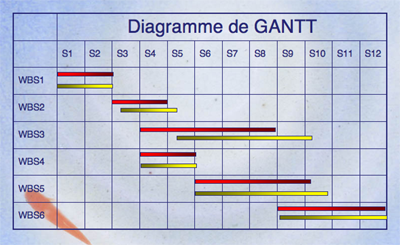
\includegraphics[width=13cm]{Gantt.png}
		\caption{Planning.}
	\label{fig:gantt}
\end{figure}
		

\subsection{Location }
The project will take place in the project room EEA of building SP2MI.
\end{document}



